\documentclass[a4paper]{article} 
\addtolength{\hoffset}{-2.25cm}
\addtolength{\textwidth}{4.5cm}
\addtolength{\voffset}{-3.25cm}
\addtolength{\textheight}{5cm}
\setlength{\parskip}{0pt}
\setlength{\parindent}{0in}

\usepackage[square,sort,comma,numbers]{natbib}
\usepackage{blindtext} % Package to generate dummy text
\usepackage{charter} % Use the Charter font
\usepackage[utf8]{inputenc} % Use UTF-8 encoding
\usepackage{microtype} % Slightly tweak font spacing for aesthetics
\usepackage{amsthm, amsmath, amssymb} % Mathematical typesetting
\usepackage{float} % Improved interface for floating objects
\usepackage{hyperref} % For hyperlinks in the PDF
\usepackage{graphicx, multicol} % Enhanced support for graphics
\usepackage{xcolor} % Driver-independent color extensions
\usepackage{pseudocode} % Environment for specifying algorithms in a natural way
\usepackage[mmddyy]{datetime} % Uses YEAR-MONTH-DAY format for dates

\usepackage{fancyhdr} % Headers and footers
\pagestyle{fancy} % All pages have headers and footers
\fancyhead{}\renewcommand{\headrulewidth}{0pt} % Blank out the default header
\fancyfoot[L]{} % Custom footer text
\fancyfoot[C]{} % Custom footer text
\fancyfoot[R]{\thepage} % Custom footer text
\newcommand{\note}[1]{\marginpar{\scriptsize \textcolor{red}{#1}}} % Enables comments in red on margin

\DeclareMathOperator*{\argmin}{arg\,min}

%----------------------------------------------------------------------------------------


%-------------------------------
%	TITLE VARIABLES (identify your work!)
%-------------------------------

\newcommand{\yourname}{Balthazar Neveu | Jamy Lafenetre}
\newcommand{\youremail}{balthazarneveu@gmail.com | jamy.lafenetre@ens-paris-saclay.fr}
\newcommand{\assignmentnumber}{2}

\begin{document}

%-------------------------------
%	TITLE SECTION (do not modify unless you really need to)
%-------------------------------
\fancyhead[C]{}
\hrule \medskip
\begin{minipage}{0.295\textwidth} 
\raggedright
\footnotesize
\yourname \hfill\\
\youremail
\end{minipage}
\begin{minipage}{0.4\textwidth} 
\centering 
\large 
Lab session \# \assignmentnumber\\ 
\normalsize 
NPM 2024\\ 
\end{minipage}
\begin{minipage}{0.295\textwidth} 
\raggedleft
\today\hfill\\
\end{minipage}
\medskip\hrule 
\bigskip




%-------------------------------
%	ASSIGNMENT CONTENT (add your responses)
%-------------------------------


\section{Question 1: ICP}
\begin{figure}[ht]
    \centering
    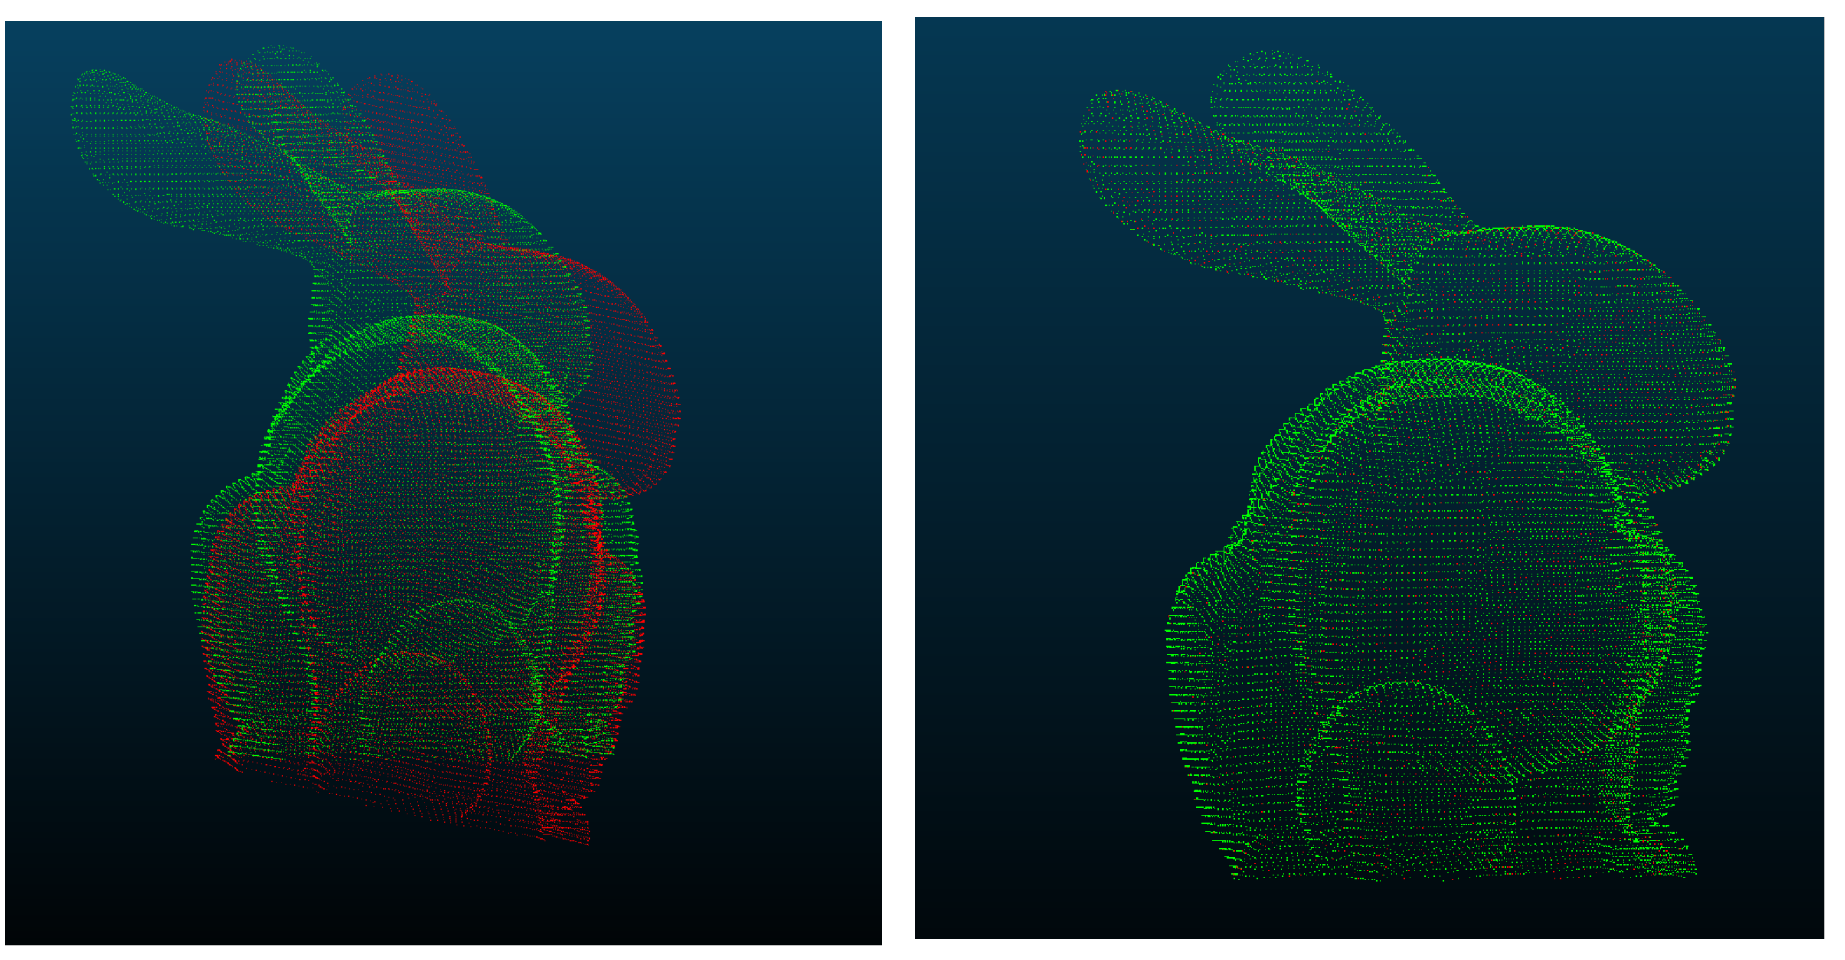
\includegraphics[width=0.8\linewidth]{figures/bunny_icp_cloud_compare.png}
    \caption{Left: reference cloud in green (template to match), misaligned candidate cloud in red. Right: After ICP alignment in Cloud Compare, $\text{RMSE}=7.2. 10^{-8}$}
    \label{fig:CC_alignment_ok}
\end{figure}

\begin{figure}[ht]
    \centering
    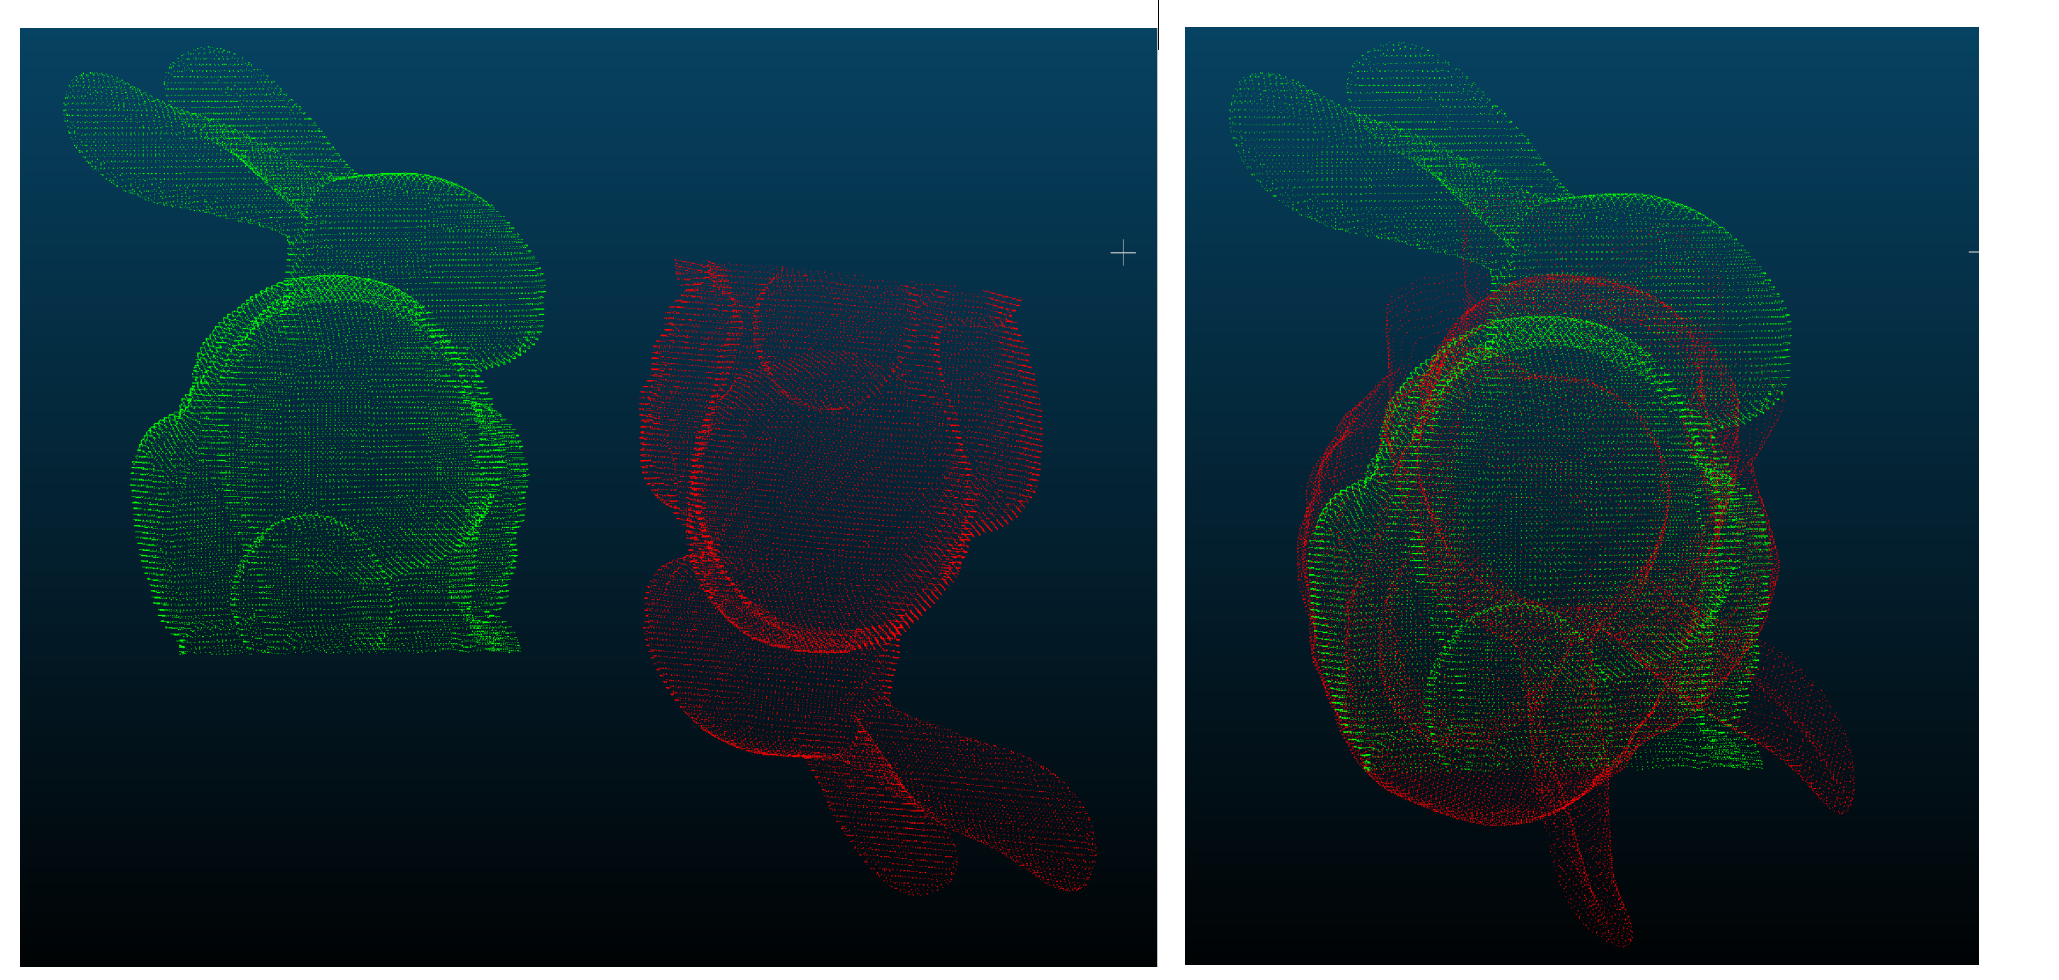
\includegraphics[width=0.8\linewidth]{figures/bunny_icp_upside_down_cloud_compare.png}
    \caption{Left: reference cloud in green (template to match), misaligned candidate cloud in red (upside down initialization). 
    Right: After ICP alignment in Cloud Compare, root mean squared error $\text{RMSE}=0.013$}
    \label{fig:CC_alignment_nok}
\end{figure}

The ICP algorithm is very sensitive to initialization. For the bunny example (same geometry without noise), two different initializations provide very different results.
Figure ~\ref{fig:CC_alignment_ok} shows a nearly perfect alignment, while Figure ~\ref{fig:CC_alignment_nok} shows a bad alignment probably due getting stuck in a local minimum.

\begin{figure}[ht]
    \centering
    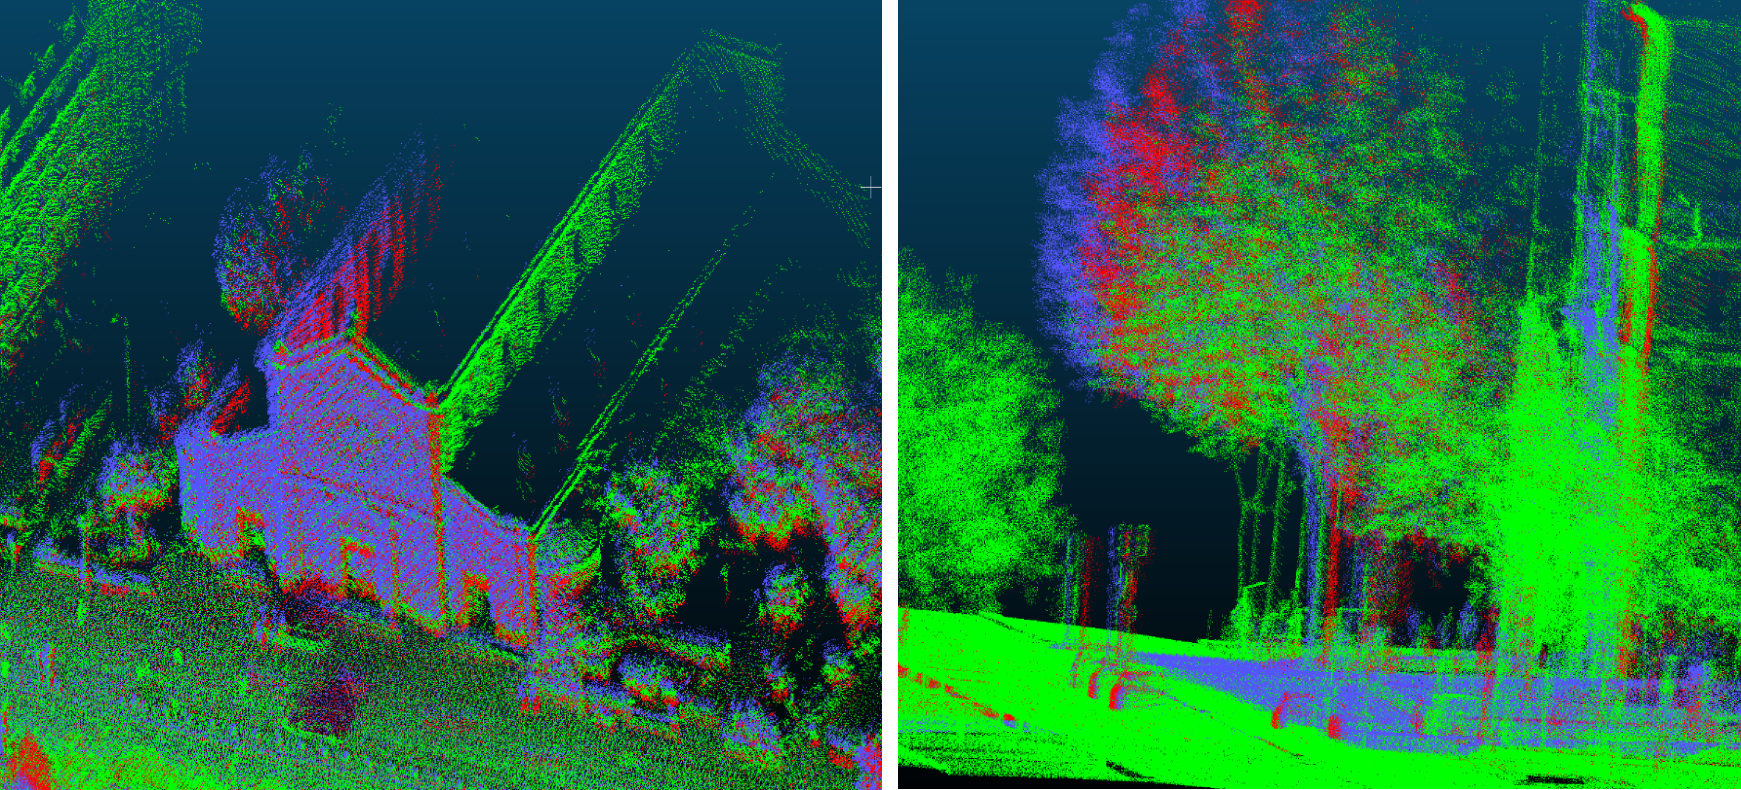
\includegraphics[width=0.8\linewidth]{figures/notre_dame_des_champs_registration.png}
    \caption{Reference cloud in green - the largest cloud, misaligned candidate cloud in blue and ICP registration result in blue $\text{RMSE}=1.39$. We're off by more than a meter in average after alignment,
    we observe that objects have moved between these scenes so without outlier removal, we can't naturally expect a perfect alignment no matter the quality of the registration algorithm.}
    \label{fig:CC_notredame}
\end{figure}
The estimated transformation matrix is quite close to the identity matrix since the misaligned was not pretty tiny. Seems like most of the misalignment source came from the ground not being perfectly aligned (the blue ground is not horizontal in figure ~\ref{fig:CC_notredame_z})
\begin{verbatim}
  Transformation matrix - Scale: fixed (1.0)
  0.999	0.008	0.032	6.017
  -0.010	0.998	0.060	-8.688
  -0.031	-0.060	0.998	-67.759
  0.000	0.000	0.000	1.000
\end{verbatim}

\begin{figure}[ht]
    \centering
    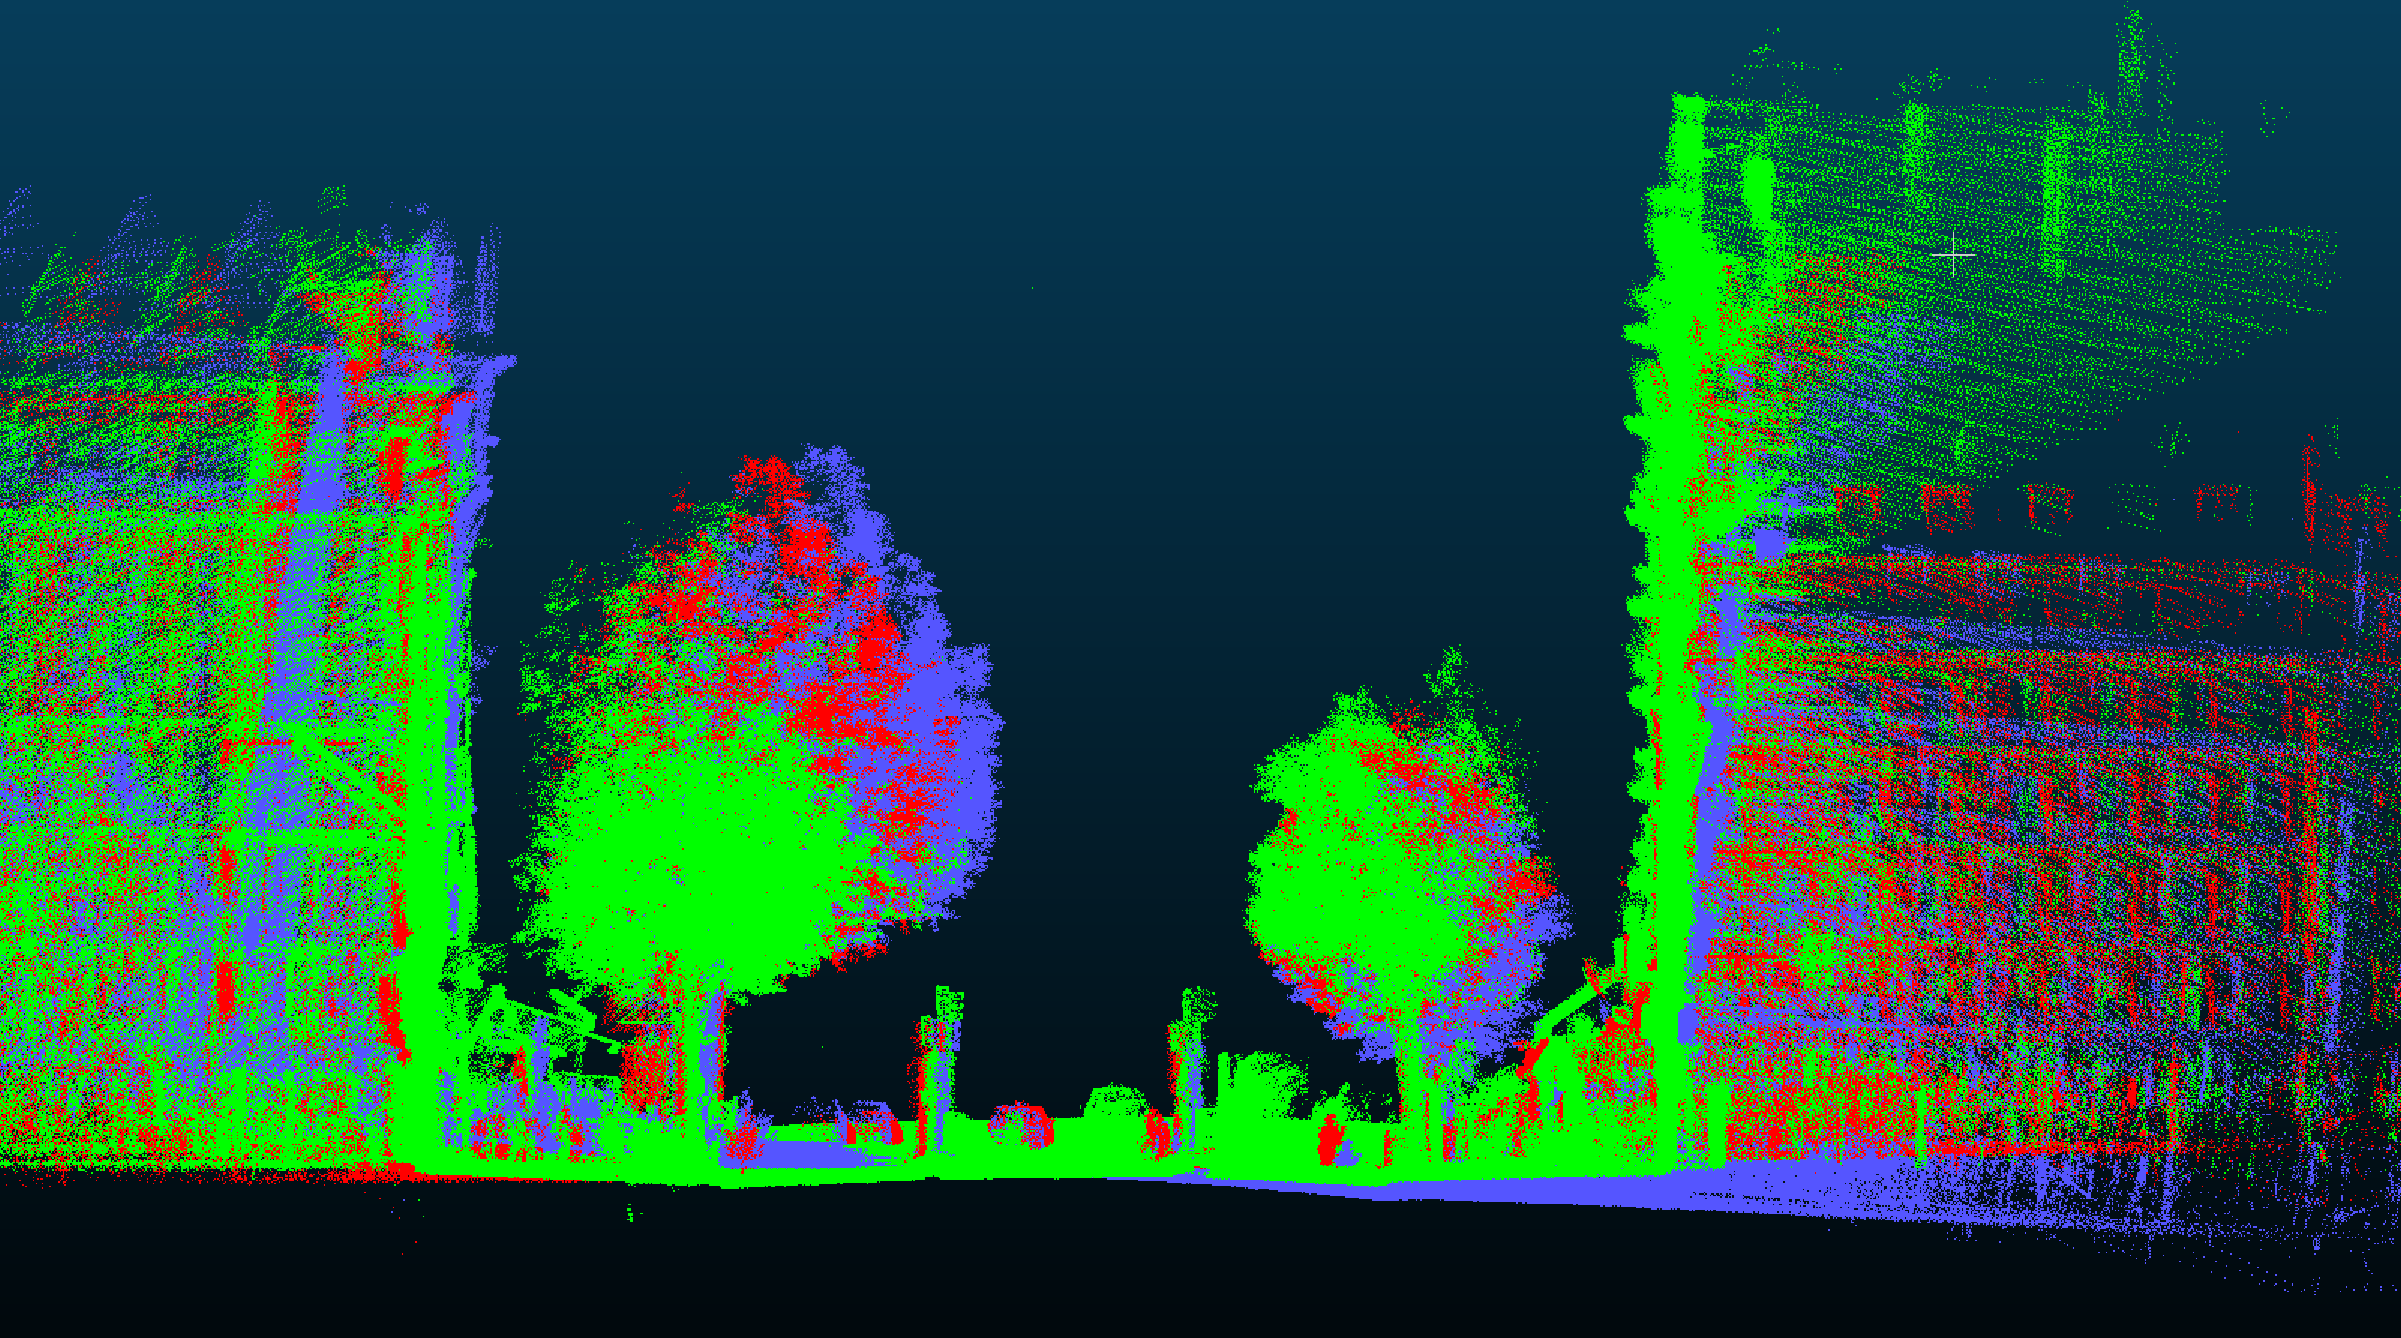
\includegraphics[width=0.8\linewidth]{figures/notre_dame_des_champs_registration_rotation.png}
    \caption{Most of the misalignment seem to have been on the Z axis - ground is not horizontal in the blue misaligned scene.}
    \label{fig:CC_notredame_z}
\end{figure}
\textbf{We use the largest cloud as reference cloud (Notre dame des champs 1).} It seems more natural as the small candidate cloud can potentially match all its points to the bigger reference cloud (this does not work the other way around).
\section{Question 2: Rigid transformation estimation}
\begin{itemize}
  \item 2 sets of matched points, $\text{RMS} = 0.$.
Works perfectly because the input points are perfectly matched (no noise) and we use a closed form solution for the rigid transformation estimation.
  \item ICP struggles because of a bad initialization and gets stuck in a local minimum (translation is not too bad).
\end{itemize}


For the real scene "Notre Dame des champs", we do not even know if the points are matched (we don't have the same amount of points.) 


% \begin{figure}[ht]
%     \centering
%     \includegraphics[width=0.5\linewidth]{figures/temperature_sampling.png}
%     \caption{Random sampling on the distribution using the temperature parameter. Temperature = 0 is equivalent to the argmax sampling.}
%     \label{fig:random_sampling}
% \end{figure}



\end{document}